\section{The rusty screw}

\begin{center}
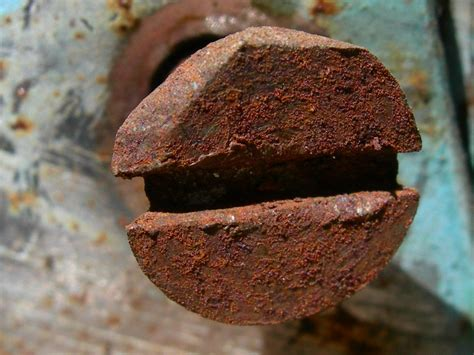
\includegraphics[width=7cm]{images/17_screw.jpg}
\end{center}

\textit{What does Tantra have to do with sex again?}

We are not mainstream and most Tantra schools put their emphasis on other topics. It's not good for business: after all, sex sells. It is not even easy to comprehend for many as "Tantra has much to do with closeness, touch, intimacy, thus sex, right?!"

It's irritating for those who have shown off their joy for desire like a hip accessory which states "Tantra". And now it is gone! Quickly it is not simply about the joy of lust anymore, but it is more noble sounding and close to enlightenment. It is not that joyful anymore, but instead the flawless strive for universal unity reveals itself.

We say it again, and we will say it every time: \textbf{Tantra only has to do with sex marginally}.

There is nothing wrong with pure lust and joyful fuckery is nice. But it is not the goal of Tantra. So why do we deal with the body, feelings, energies, exploration, discovery and the healing of our sexuality at retreats anyhow, if it is supposed to have nothing to do with Tantra? Because Tantra uses the most original of all energies, in order to develop mindfulness, insight, patience and the slow detachment of the ego. This primordial energy is available within us in huge amounts, and we can tap into it the most easily through joy which we experience with increasing erotic tension.

Most of us have no unbiased access to this energy source due to upbringing, social imprint, personal history, \ldots That's why Western Tantra aims at smoothing out the deformations in this area during the first stages: Fears, trauma, role models, prejudgements, \ldots

The exercises which are being offered are not means to their own end, and if you succeed in an exercise, you are not there yet, you haven’t reached the goal, because the goal of Tantra is not an easy going attitude to sexuality. An easy going attitude to sexuality is rather the precondition for Tantra.

The exercises at a retreat are more like supporting wheels, just like young kids use them when they want to learn how to ride a bicycle: Once they feel safe enough to sit in the saddle by themselves, they don't need the supporting wheels anymore. The same applies here: Once the goal of total insight is achieved, the exercises become unnecessary.

Just take, for example, a rusty screw, which is mounted wrongly and wobbly, and can do its job only half-heartedly. In order for it to be mounted properly again, we first need to free it from the rust. That can be effortful and take a long time. Yet, only few will think that cleaning off the rust is the actual goal. At the end, it is about the screw itself and as soon as the rust is gone, it can be screwed in nicely again and we stop cleaning it.

Thus, in Tantra it is not about a better, more amazing, exciting, \ldots sexuality. It is about making this primary, creative, potent energy accessible (with lots of discipline, by the way) and about using it as a vehicle to achieve the actual Tantric goals: Ever deepened awareness, mindfulness, loving kindness and serenity in every situation.
